\section{Empirical Evaluation}
\label{sec:evaluation}

\subsection{Research questions}

These seem quite pertinent to the overall problem of transparent science communication:
\begin{itemize}
\item How does performance degrade with partial/ambiguous information?
\item How is performance affected by ``adversarial'' (intentionally/unintentionally misleading) information?
\end{itemize}

Some ways we might explore these axes:
\begin{itemize}
\item meaningful vs.~meaningless vs.~misleading identifiers
\item leaving out key criteria (e.g.~year) that would resolve query to unique answer
\end{itemize}

We might want to distinguish ambiguity inherent in the problem domain (e.g.~uncertainty) vs.~ambiguity in the
specification of a particular code-generation query.

\subsection{Success Rate by Category}
To evaluate the system we used a sample of the Scigen dataset~\citep{scigen_dataset_2021}.

We aggregated the generated expression in three categories: aggregation, trends, quantitative (See Table \ref{tab:fluid_examples}).
Figure \ref{fig:success_rate_by_category} shows the results obtained in generating expression by categories.

\begin{figure}
    \centering
    \begin{subfigure}{0.48\linewidth}
        \centering
        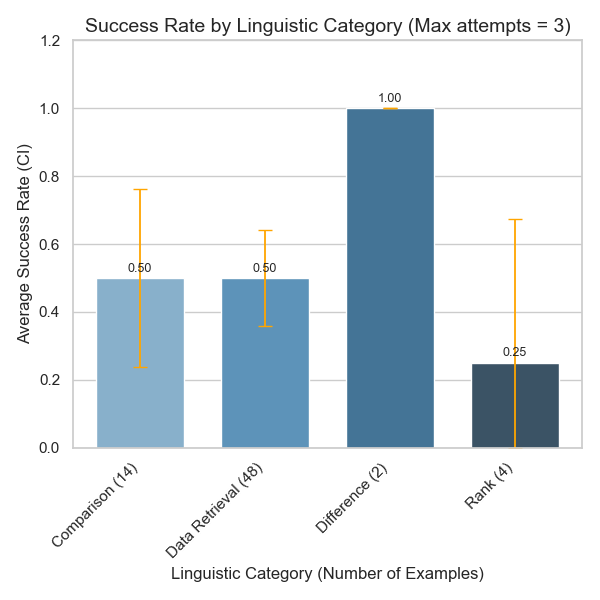
\includegraphics[width=\linewidth]{fig/success_rate_by_category}
        \caption{Success rate by testcases}
        \label{fig:success_rate_by_category}
    \end{subfigure}\hfill
    \begin{subfigure}{0.48\linewidth}
        \centering
        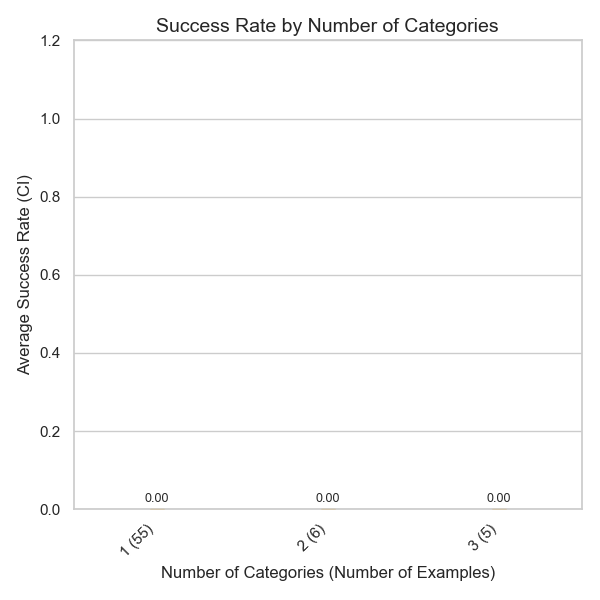
\includegraphics[width=\linewidth]{fig/success_rate_by_category_count}
        \caption{Success rate by category count}
        \label{fig:success_rate_by_category_count}
    \end{subfigure}
    \caption{Comparison of success rates}
    \label{fig:success_rate_comparison}
\end{figure}
